% Semantics-Driven Visual Reduction for Building Knowledge Graphs
% Draft academic paper describing the design of 223p-viewer.
% Build: pdflatex paper && bibtex paper && pdflatex paper && pdflatex paper
% Uses only standard packages so it can be dropped into a venue template
% (ACM acmart / IEEE conference) by swapping the \documentclass line.

\documentclass[10pt,twocolumn]{article}
\usepackage[margin=0.75in]{geometry}
\usepackage[T1]{fontenc}
\usepackage{lmodern}
\usepackage{microtype}
\usepackage{graphicx}
\usepackage{booktabs}
\usepackage{amssymb}
\usepackage{xcolor}
\usepackage{tikz}
\usetikzlibrary{arrows.meta,positioning}
\usepackage{enumitem}
\usepackage[hidelinks]{hyperref}
\usepackage{cleveref}

\newcommand{\pred}[1]{\texttt{#1}}   % RDF predicate / class name
\newcommand{\todo}[1]{\textcolor{red}{[TODO: #1]}}

\title{One Building, Many Mental Models:\\
Semantics-Driven Views of ASHRAE 223P and Brick Building Models}

% TODO: confirm author list, ordering, and affiliations before submission.
\author{Lazlo Paul\\
University of California, Berkeley\\
\texttt{lazlopaul@berkeley.edu}}

\date{Draft --- October 2026}

\begin{document}
\maketitle

\begin{abstract}
Semantic building models expressed in RDF---notably ASHRAE Standard 223P and the
Brick schema---encode equipment, physical connectivity, containment, sensing, and
control in a machine-readable graph. Those same models are notoriously hard for
people to \emph{look at}: a modest office-building model contains thousands of
triples, and a real building tens of thousands, most of which are scaffolding
(connection points, connection hubs, quantity kinds, units) rather than things an
engineer would draw. Generic RDF and ontology visualizers render that scaffolding
faithfully and therefore overwhelm the user. We argue that the underlying problem
is one of \emph{alignment}: a useful view matches the digital representation to
the mental model its user brings, and different users bring different ones---an
inventory of what kinds of things the model contains, the physical topology of
how the building is put together, and the data-and-control picture of what can be
measured and commanded. A rich semantic model is valuable precisely because it
holds enough information to serve all of these at once. We present
\emph{223p-viewer}, a browser-based visualizer that serves each mental model as a
separate but connected \emph{lens} over one shared domain model, and uses the
ontology's own semantics to decide what each lens draws, what it folds away, and
what it defers until asked for. We relate the lenses to the coverage of common
building ontologies (223P, Brick, Haystack, RealEstateCore, BOT/IFC, SOSA/SSN).
We describe seven semantic reduction techniques (including
hub-chain collapse, connection points as port glyphs, containment-driven drill-down,
and edge roll-up to the nearest visible ancestor), a progressive-disclosure
overlay for the sensing-and-control layer, a schema-summary entry point, and a
query-construction workflow that turns what is on screen into structured triples
for downstream SPARQL. On a 1{,}707-triple reference model the root view shows 25
boxes and 45 arrows; on a 38{,}982-triple real building it shows 143 boxes and 320
arrows---still dense, which we report as a limitation. We also report negative
results: three abandoned designs for rendering logical \pred{System} groupings, and
reverted name-based heuristics. We distill these into design principles for
semantic building-model visualization, chief among them that \emph{one model should serve
many mental models through connected lenses}, that \emph{one tree should be
governed by one relation}, and that \emph{nothing should vanish silently}.
\end{abstract}

% ---------------------------------------------------------------------------
\section{Introduction}

Buildings account for a large share of energy use, and most analytics,
fault-detection, and supervisory-control applications for them are written once
per building because the metadata describing \emph{what is connected to what}
lives in inconsistent point names and drawings. Semantic models attack that
problem directly. Brick~\cite{balaji2016brick} provides a vocabulary of
equipment, points, and locations; ASHRAE Standard 223P~\cite{ashrae223p} goes
further and models physical topology explicitly, down to the connection points on
each piece of equipment, the ducts, pipes, and conductors between them, the
properties those connections carry, and the sensors that observe them. A
review by Pritoni et al.~\cite{pritoni2021metadata} surveys this landscape.

This expressiveness has a cost that falls on humans. Modelers need to verify that
a model is right; integrators need to find the handful of entities an application
needs; researchers need to understand an unfamiliar building. All of them
eventually want to \emph{see} the model. But the literal graph is the wrong thing
to show. In 223P a single duct from an air-handling unit (AHU) to a VAV box is at
least five nodes and four edges (equipment, outlet connection point, connection,
inlet connection point, equipment), and every property hangs further nodes for its
quantity kind and unit. A force-directed drawing of every triple---what a generic
RDF browser produces---is a hairball long before the building is interesting.

The literal graph is also the wrong thing to show because there is no single
right thing to show. People understand a building through a \emph{mental
model}~\cite{johnsonlaird1983mental,norman2013design}, and the people who use
semantic models hold different ones. An integrator writing a portable analytics
query thinks in \emph{kinds}: which classes of equipment and points exist, and how
many. A mechanical designer or commissioning agent thinks in \emph{topology}: this
fan pushes air through that duct into that box. A controls engineer or
fault-detection analyst thinks in \emph{data}: which sensor observes which
property, and which command drives which actuator. These are not competing
interpretations to be reconciled into one picture; they are different questions
asked of the same building. 223P is verbose largely \emph{because} it carries the
information for all of them at once: ports and connections for topology,
properties and instrumentation for data, classes for inventory.

This paper documents the approaches we took in building \emph{223p-viewer}, an
open-source, client-only visualizer for 223P (and, through the same pipeline,
Brick) models. It rests on two ideas. First, \textbf{serve each mental model as
its own lens over one shared model, and keep the lenses connected}, so that a user
can start from the view that matches how they think and cross into another
without losing their place. Second, \textbf{the ontology already tells us what the
domain's ``things'' are, how they nest, and which relations are scaffolding}, so
each lens should use that semantics to reduce the graph before any layout
algorithm sees it, and then reveal the rest progressively.
Concretely, we contribute:

\begin{enumerate}[leftmargin=*,itemsep=1pt]
  \item A framing of semantic-model visualization as \emph{mental-model
  alignment}, three connected lenses (inventory, topology, data-and-control)
  that realize it, and an analysis of which lenses common building ontologies
  can support (\cref{sec:lenses}).
  \item A catalog of \emph{semantic reduction} techniques for 223P/Brick, each a
  domain-justified mapping from RDF patterns to visual marks
  (\cref{sec:reduction}).
  \item A \emph{progressive disclosure} design for the sensing-and-control layer,
  a schema-summary entry point, and a view-scoped query-construction workflow
  (\cref{sec:disclosure}).
  \item Layout and responsiveness techniques that matter specifically for
  real building data (\cref{sec:layout}).
  \item A design-history case study of logical \pred{System} groupings,
  including three abandoned approaches (\cref{sec:systems}).
  \item Design principles distilled from the above, and a descriptive
  evaluation on four bundled models that is candid about where the approach
  still overwhelms (\cref{sec:principles,sec:eval,sec:limits}).
\end{enumerate}

% ---------------------------------------------------------------------------
\section{Background and Related Work}
\label{sec:related}

\paragraph{Semantic building models.}
Brick~\cite{balaji2016brick} models equipment, points, and spaces with a compact
relation set (\pred{feeds}, \pred{hasPoint}, \pred{hasPart},
\pred{hasLocation}). ASHRAE 223P~\cite{ashrae223p} models physical topology:
equipment owns typed connection points (\pred{hasConnectionPoint}, inlet/outlet/
bidirectional), which are joined through \pred{Connection} entities
(\pred{Duct}, \pred{Pipe}, \pred{Conductor}) via \pred{cnx} or
\pred{connectsThrough}; containment is \pred{contains}/\pred{encloses};
\pred{System} and \pred{Zone} group members via \pred{hasMember} and
\pred{hasDomainSpace}; and an instrumentation layer relates sensors, actuators,
and functions to properties and locations (\pred{observes},
\pred{actuatedByProperty}, \pred{hasInput}/\pred{hasOutput},
\pred{hasObservationLocation}, \pred{executes}).

\paragraph{Ontology and RDF visualization.}
General-purpose tools such as VOWL~\cite{lohmann2016vowl} visualize ontology
\emph{schemas} (classes and properties); RDF browsers visualize instance graphs
generically. Neither knows that a 223P connection point is ``a port on a box'' or
that a \pred{Connection} is ``an arrow''. Our work is deliberately the opposite
trade-off: it hard-codes one family of ontologies to gain domain-faithful,
low-clutter views.

\paragraph{Mental models and multiple views.}
Users form mental models of a system and act through them; a display succeeds
when its conceptual model matches the user's~\cite{johnsonlaird1983mental,norman2013design}.
Process-control research made this concrete for engineered plants:
Rasmussen's abstraction hierarchy describes the same plant at several levels, from
purpose and function down to physical form~\cite{rasmussen1985role}, and
ecological interface design builds operator displays around those
levels~\cite{vicente1992ecological}. Our lenses are a lightweight instance of the
same idea for building models. The visualization literature on coordinated
multiple views~\cite{wangbaldonado2000guidelines,roberts2007state} supplies the
mechanics: several views of one dataset, linked so that a selection or
navigation in one carries into the others.

\paragraph{Large-graph visualization.}
The classic mantra ``overview first, zoom and filter, then details on
demand''~\cite{shneiderman1996eyes} and degree-of-interest
techniques~\cite{furnas1986fisheye,vanham2009search} motivate our progressive
disclosure. Hierarchical aggregation~\cite{elmqvist2010hierarchical,abello2006askgraphview}
and the broader graph-navigation literature~\cite{herman2000graph} motivate our
drill-down and edge roll-up. Our layout builds on layered (Sugiyama-style)
drawing~\cite{sugiyama1981methods,gansner1993technique} via the dagre library.
What distinguishes our setting is that the aggregation hierarchy is not inferred
by clustering; it is \emph{given} by the ontology's containment relations---and
the ontology also supplies competing, non-tree groupings (\pred{System}) that must
be reconciled with it (\cref{sec:systems}).

% ---------------------------------------------------------------------------
\section{One Model, Several Mental Models}
\label{sec:lenses}

\Cref{tab:lenses} summarizes the three lenses 223p-viewer provides. Each answers a
different question, serves a different user, and puts different parts of the same
model in focus while demoting the rest to context.

\begin{table*}[t]
\centering
\small
\caption{Three mental models served as three connected lenses over one domain
model.}
\label{tab:lenses}
\begin{tabular}{p{2.6cm}p{4.0cm}p{4.0cm}p{4.6cm}}
\toprule
 & \textbf{Inventory} & \textbf{Topology} & \textbf{Data \& control} \\
\midrule
Question & What \emph{kinds} of things are in this model, and how many? &
How is the building put together, and what is connected to what? &
What can be measured and commanded, and where? \\
Typical user & Integrator, analytics developer, modeler auditing consistency &
Mechanical designer, commissioning agent, operator tracing a flow path &
Controls engineer, fault-detection analyst \\
In focus & Structural classes and their member counts & Equipment, ports,
connections, containment & Sensors, actuators, functions, properties and values \\
Demoted to context & Individual instances (listed on hover) & Properties
(tooltips), instrumentation (hidden) & Equipment without data (muted) \\
In 223p-viewer & BSchema view (\cref{fig:bschema}) & Equipment view
(\cref{fig:root}) & Sensors \& Controls overlay (\cref{fig:overlay}) \\
\bottomrule
\end{tabular}
\end{table*}

\paragraph{Connected, not merged.}
The lenses are useful because they are separate and because they are linked. They
share one domain model (\cref{sec:overview}), so an entity has the same identity
(its URI) in every lens, and crossing between lenses is cheap:
\begin{itemize}[leftmargin=*,itemsep=1pt]
  \item \emph{Inventory $\to$ topology.} Each summary class lists its real
  members; clicking one opens the instance view drilled to the member's
  container, with the member highlighted and the data overlay on.
  \item \emph{Topology $\leftrightarrow$ data.} The data lens is an overlay on the
  topology lens's own containment tree, not a separate canvas. An earlier version
  had a separate, flat ``points'' canvas; it answered \emph{what sensors exist}
  but lost \emph{where they are}, which is exactly what the topology lens supplies.
  \item \emph{Any lens $\to$ query.} The query-selection clipboard draws from
  whatever the current lens shows (\cref{sec:disclosure}), so each mental model
  is also a starting point for a SPARQL query.
\end{itemize}

\paragraph{Served differently.}
Because the lenses are independent views over one model, they need not be
delivered together. In the standalone app they are tabs and a toggle; in the
notebook widget, an analyst gets the topology lens plus a triple-export clipboard
and no inventory tab. A facilities tool could open on the data lens and a
design-review tool on the topology lens. Choosing a lens is a deployment choice,
not a change to the model.

\paragraph{What the ontology must contain.}
A lens can only be served if the ontology records the information it needs.
\Cref{tab:ontologies} compares common building ontologies against the three lenses
plus spatial context. This is an analytical comparison: 223p-viewer implements
223P and Brick, and the other rows describe what a lens over each would have to
work with.

\begin{table*}[t]
\centering
\small
\caption{Which mental models common building ontologies can support. \checkmark{}
= first-class constructs; $\circ$ = partial or coarse; -- = out of scope.
223p-viewer currently reads 223P and Brick.}
\label{tab:ontologies}
\begin{tabular}{p{2.5cm}p{3.1cm}p{3.6cm}p{3.6cm}p{3.1cm}}
\toprule
Ontology & Inventory & Topology & Data \& control & Spatial context \\
\midrule
ASHRAE 223P~\cite{ashrae223p} & \checkmark{} class hierarchy &
\checkmark{} connection points, \pred{Connection}s, \pred{cnx} &
\checkmark{} \pred{Property}, \pred{observes}, actuators, functions &
\checkmark{} physical and domain spaces, zones \\
Brick~\cite{balaji2016brick} & \checkmark{} class hierarchy &
$\circ$ \pred{feeds}, \pred{hasPart} at equipment level, no ports &
\checkmark{} Points (sensor, setpoint, command), \pred{hasPoint} &
\checkmark{} locations, \pred{hasLocation} \\
Project Haystack~\cite{haystack} & $\circ$ tags and defs &
$\circ$ references are mostly ownership and siting &
\checkmark{} point tags, \pred{equipRef} & \checkmark{} \pred{siteRef}, \pred{spaceRef} \\
RealEstateCore~\cite{hammar2019rec} & \checkmark{} class hierarchy &
$\circ$ assets and components & $\circ$ points &
\checkmark{} buildings, levels, rooms \\
BOT~\cite{rasmussen2021bot} / IFC~\cite{ifc} & \checkmark{} element classes &
$\circ$ IFC distribution ports; BOT element adjacency &
-- elements, not data points & \checkmark{} site, building, storey, space \\
SOSA/SSN~\cite{haller2019ssn} & -- & -- &
\checkmark{} \pred{Sensor}, \pred{observes}, \pred{Actuator} &
$\circ$ feature of interest \\
QUDT~\cite{qudt} & -- & -- & $\circ$ units and quantity kinds on values & -- \\
\bottomrule
\end{tabular}
\end{table*}

Two observations follow. First, the ontologies are largely complementary: spatial
ontologies (BOT, IFC, RealEstateCore) are strongest where equipment and data
ontologies are weakest, and 223P is unusual in covering topology at port level.
Second, a lens degrades gracefully when its input is coarse rather than
disappearing. Our Brick support is a working example: Brick has no connection
points, so the topology lens invents one outlet/inlet pair per \pred{feeds} edge and
draws equipment-level arrows (\cref{fig:brick}), and the data lens folds Points
into equipment instead of drawing them. The same view code serves both, at the
fidelity each ontology allows.

% ---------------------------------------------------------------------------
\section{System Overview}
\label{sec:overview}

223p-viewer is a static web application (TypeScript, React, React
Flow~\cite{reactflow}) with no backend. A Turtle file is parsed in the browser
(N3.js) and passed through a single pipeline (\cref{fig:pipeline}):

\begin{figure}[t]
\centering
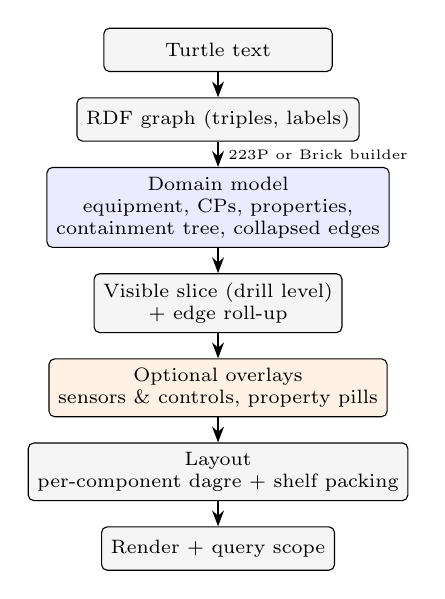
\begin{tikzpicture}[
  box/.style={draw, rounded corners=2pt, align=center, font=\scriptsize,
              minimum width=2.9cm, minimum height=0.55cm, fill=gray!8},
  arr/.style={-{Stealth[length=2mm]}, thick},
  node distance=0.32cm]
\node[box] (ttl) {Turtle text};
\node[box, below=of ttl] (rdf) {RDF graph (triples, labels)};
\node[box, below=of rdf, fill=blue!8] (model) {Domain model\\\scriptsize equipment, CPs, properties,\\\scriptsize containment tree, collapsed edges};
\node[box, below=of model] (slice) {Visible slice (drill level)\\\scriptsize + edge roll-up};
\node[box, below=of slice, fill=orange!10] (overlay) {Optional overlays\\\scriptsize sensors \& controls, property pills};
\node[box, below=of overlay] (layout) {Layout\\\scriptsize per-component dagre + shelf packing};
\node[box, below=of layout] (render) {Render + query scope};
\draw[arr] (ttl) -- (rdf);
\draw[arr] (rdf) -- node[right, font=\tiny]{223P or Brick builder} (model);
\draw[arr] (model) -- (slice);
\draw[arr] (slice) -- (overlay);
\draw[arr] (overlay) -- (layout);
\draw[arr] (layout) -- (render);
\end{tikzpicture}
\caption{Pipeline. All semantic reduction happens when building the domain
model and the visible slice, \emph{before} layout. Brick and schema-summary
graphs enter through the same domain model.}
\label{fig:pipeline}
\end{figure}

The key architectural choice is a single typed \emph{domain model} that every
view consumes: \emph{container nodes} (equipment, spaces, and---internally---hubs and
groups), \emph{connection points} with resolved owners and direction,
\emph{properties}, a single-parent containment tree, a list of collapsed
equipment-to-equipment \emph{connection edges}, and per-node
\emph{instrumentation links}. Reduction decisions are made once, in this model,
rather than independently in each view. A Brick builder produces the same shape,
so Brick models reuse every downstream component unmodified
(\cref{sec:brick}). The same pipeline is packaged as an
anywidget~\cite{anywidget} so it can be embedded in Jupyter or
marimo~\cite{marimo} notebooks.

% ---------------------------------------------------------------------------
\section{Semantic Reduction}
\label{sec:reduction}

Each technique below maps an RDF pattern that is verbose but semantically
``small'' to a compact visual mark, using only relations the standard defines.

\subsection{R1: Collapse connection hub chains into arrows}
In 223P, two pieces of equipment are connected when an outlet connection point of
one and an inlet connection point of the other are both linked (via \pred{cnx} or
\pred{connectsThrough}) to the same \pred{Connection}/\pred{Duct}/\pred{Pipe}/
\pred{Conductor}. Rather than assume exactly one hub between two points, we
union-find every connection point and hub touched by a \pred{cnx} or
\pred{connectsThrough} triple into components. Within each component, every
owned outlet is paired with every owned inlet (falling back to pairwise links when
no inlet/outlet split exists, e.g.\ bidirectional electrical points), and one
arrow is emitted per owner pair, skipping self-loops. The hub disappears as a
node but survives as the arrow's label, medium, and any properties it carries.
This handles arbitrary-length hub chains uniformly and degrades gracefully to a
direct point-to-point link. On the NIST reference model, 214
\pred{cnx}/\pred{connectsThrough} triples and 50 hub nodes become 88 arrows.

\subsection{R2: Connection points as port glyphs}
Connection points are not boxes. Each becomes a small dot on its owner's border,
inlets on the left and outlets on the right, colored by medium, with its own
hover tooltip. Arrows attach to the exact dot they connect, so a box's ports read
like a schematic symbol. Ownership is resolved from
\pred{hasConnectionPoint}, \pred{hasBoundaryConnectionPoint},
\pred{hasOptionalConnectionPoint}, and the inverse \pred{isConnectionPointOf};
when real data instead declares a port with a direct \pred{cnx} from equipment to
connection point (about one in six equipment nodes in the reference model), we
treat that as ownership too---but only as a fallback, and never for hubs, whose
\pred{cnx} edges are topology.

\subsection{R3: Properties and points live inside their owner}
\label{sec:brick}
Properties (with their value, unit symbol, quantity kind, and enumeration kind)
are listed in the owner's hover tooltip instead of being drawn as nodes. For
Brick, the same move applies to Points: anything that is the object of
\pred{hasPoint} (or subject of \pred{isPointOf}) is folded into its equipment's
property list (\cref{fig:brick}). The 72 points of the bundled Brick model
therefore add zero boxes.

\begin{figure}[t]
\centering
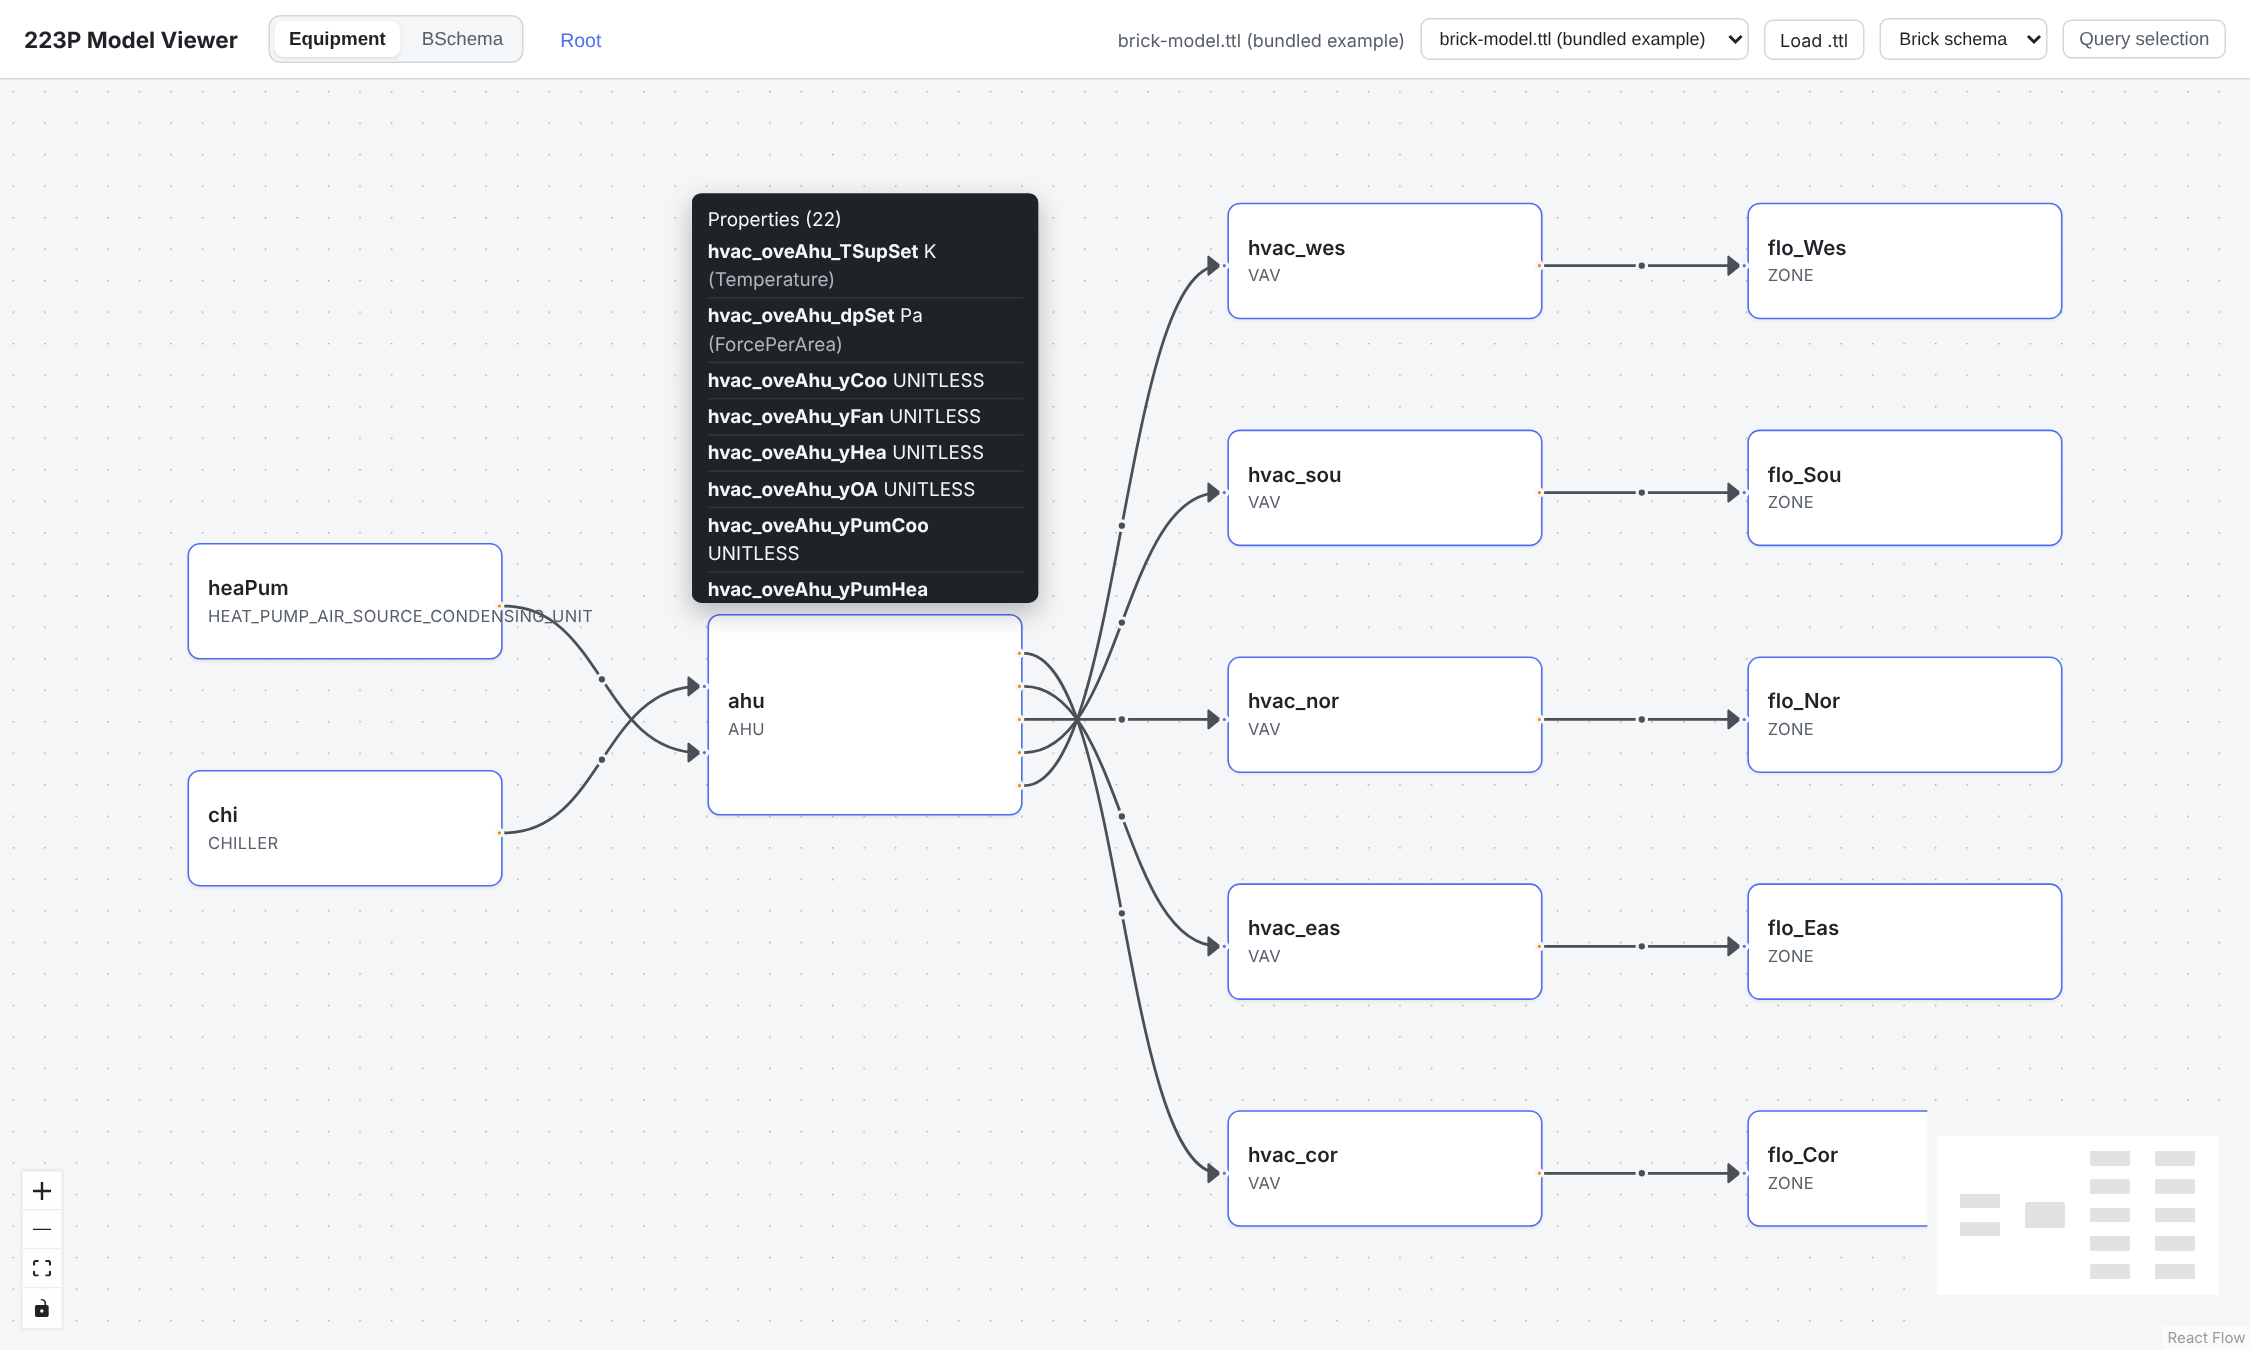
\includegraphics[width=\linewidth]{../figures/fig-brick-tooltip.png}
\caption{A Brick model through the same pipeline: \pred{feeds} becomes arrows
between synthetic ports, and the AHU's 22 \pred{hasPoint} points appear as a
property list on hover rather than 22 boxes.}
\label{fig:brick}
\end{figure}

\subsection{R4: Containment is the one drill-down hierarchy}
\pred{contains} and \pred{encloses} define a single-parent tree. The canvas shows
one level at a time: the roots, or the children of the container the user has
double-clicked into, with a breadcrumb for navigation
(\cref{fig:root,fig:drill}). This bounds what is on screen by the branching
factor of the building rather than its size.

\begin{figure*}[t]
\centering
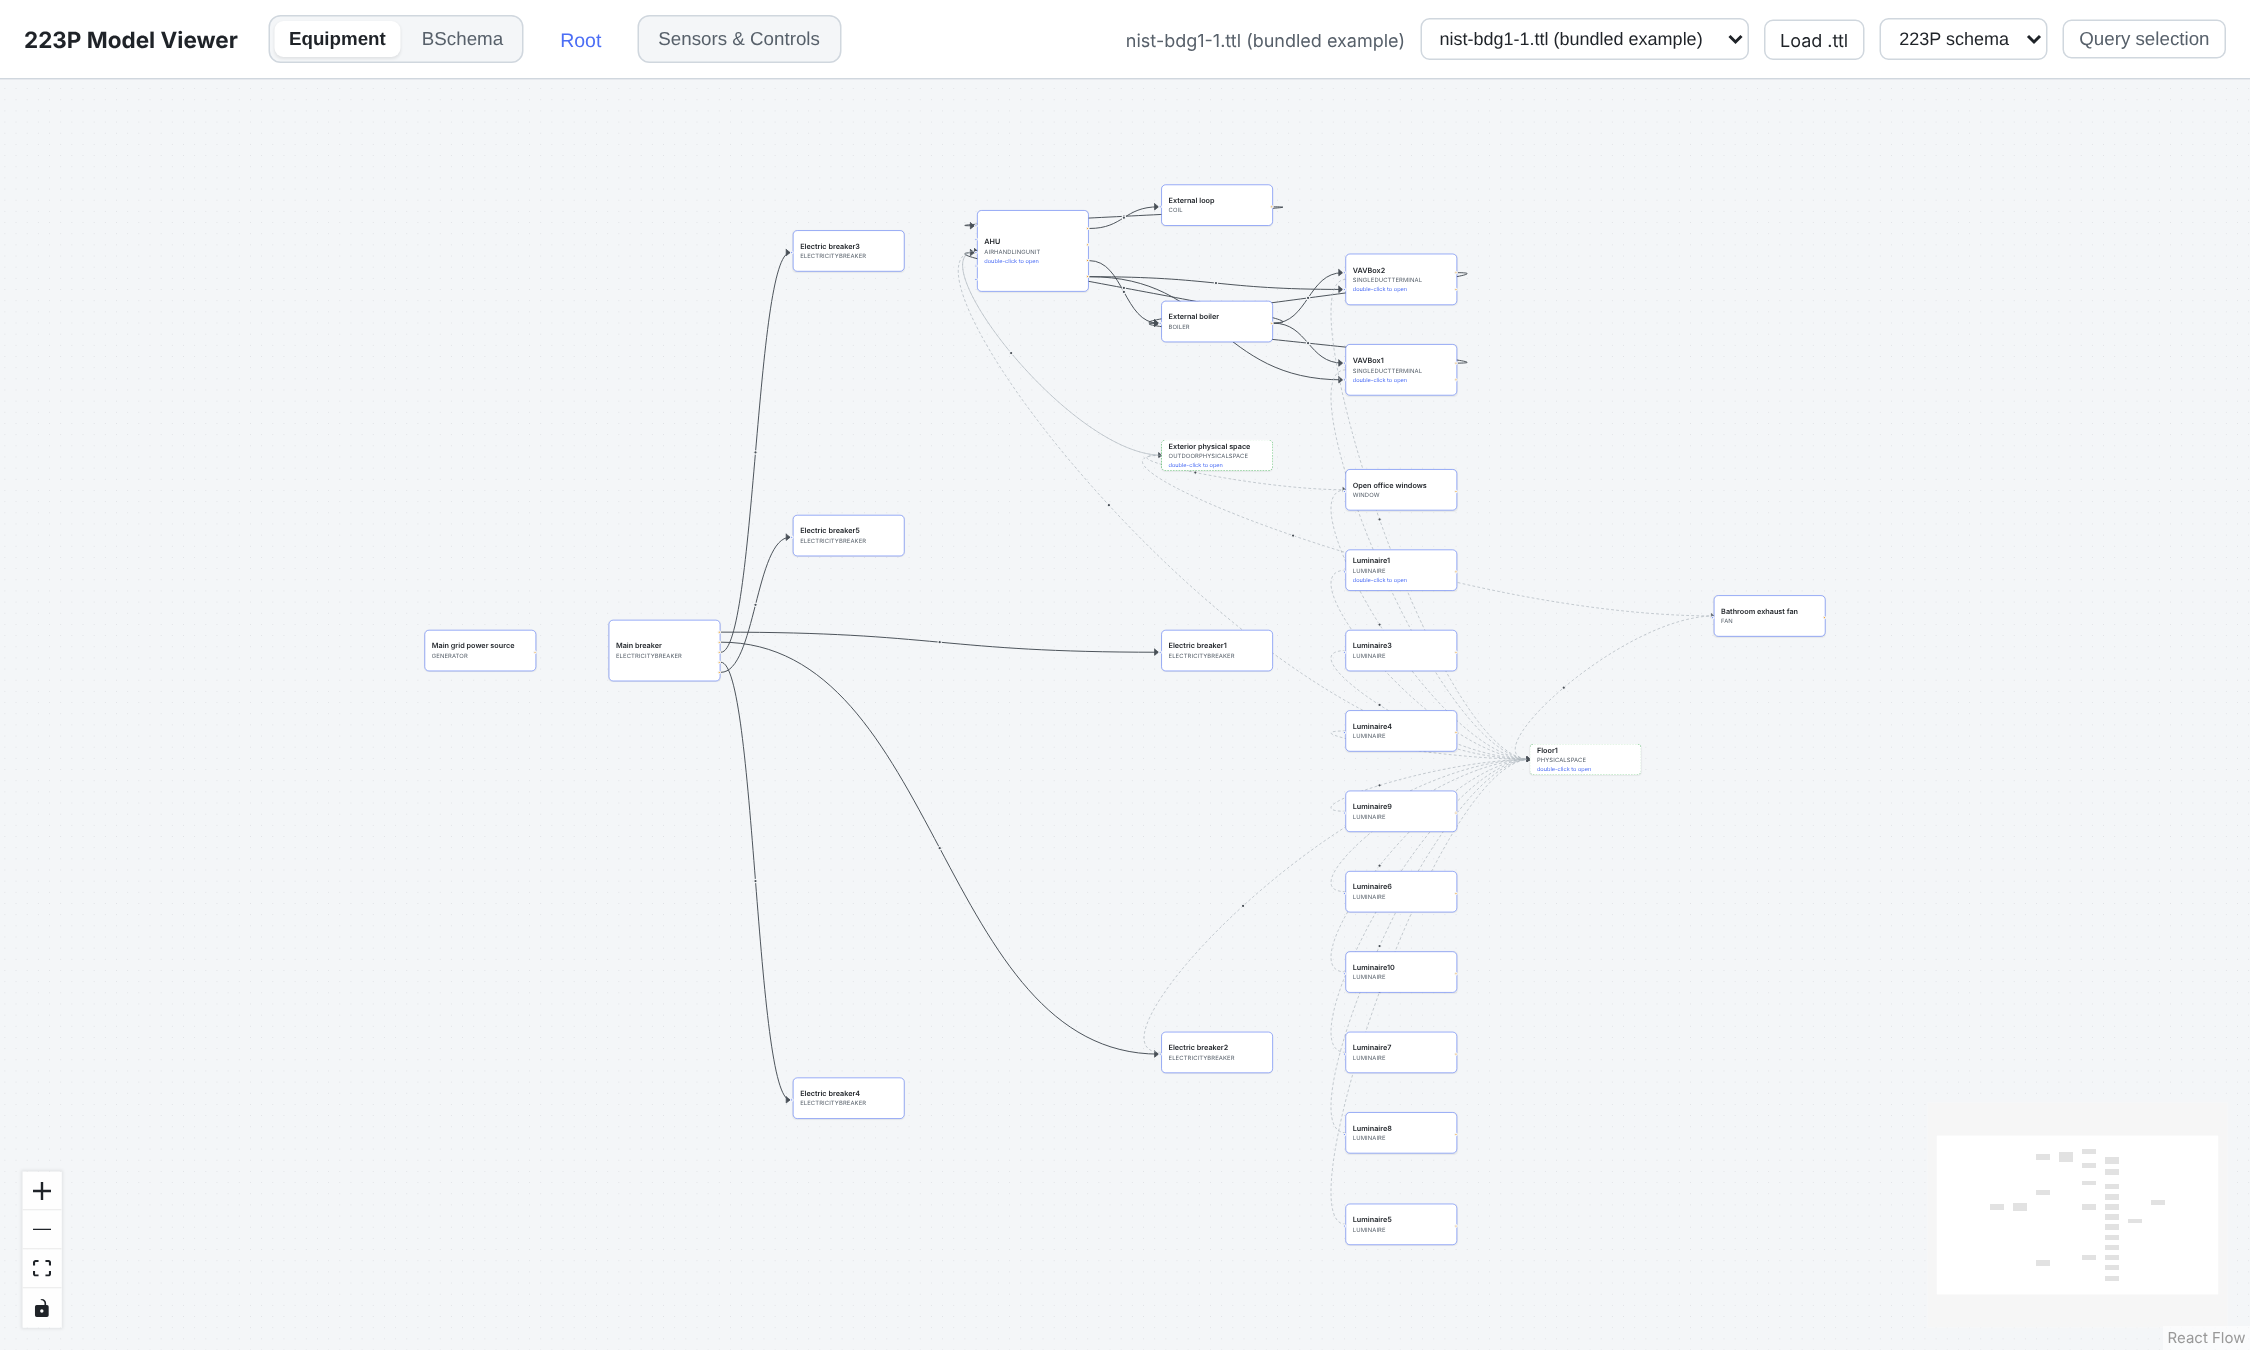
\includegraphics[width=0.49\textwidth]{../figures/fig-root.png}\hfill
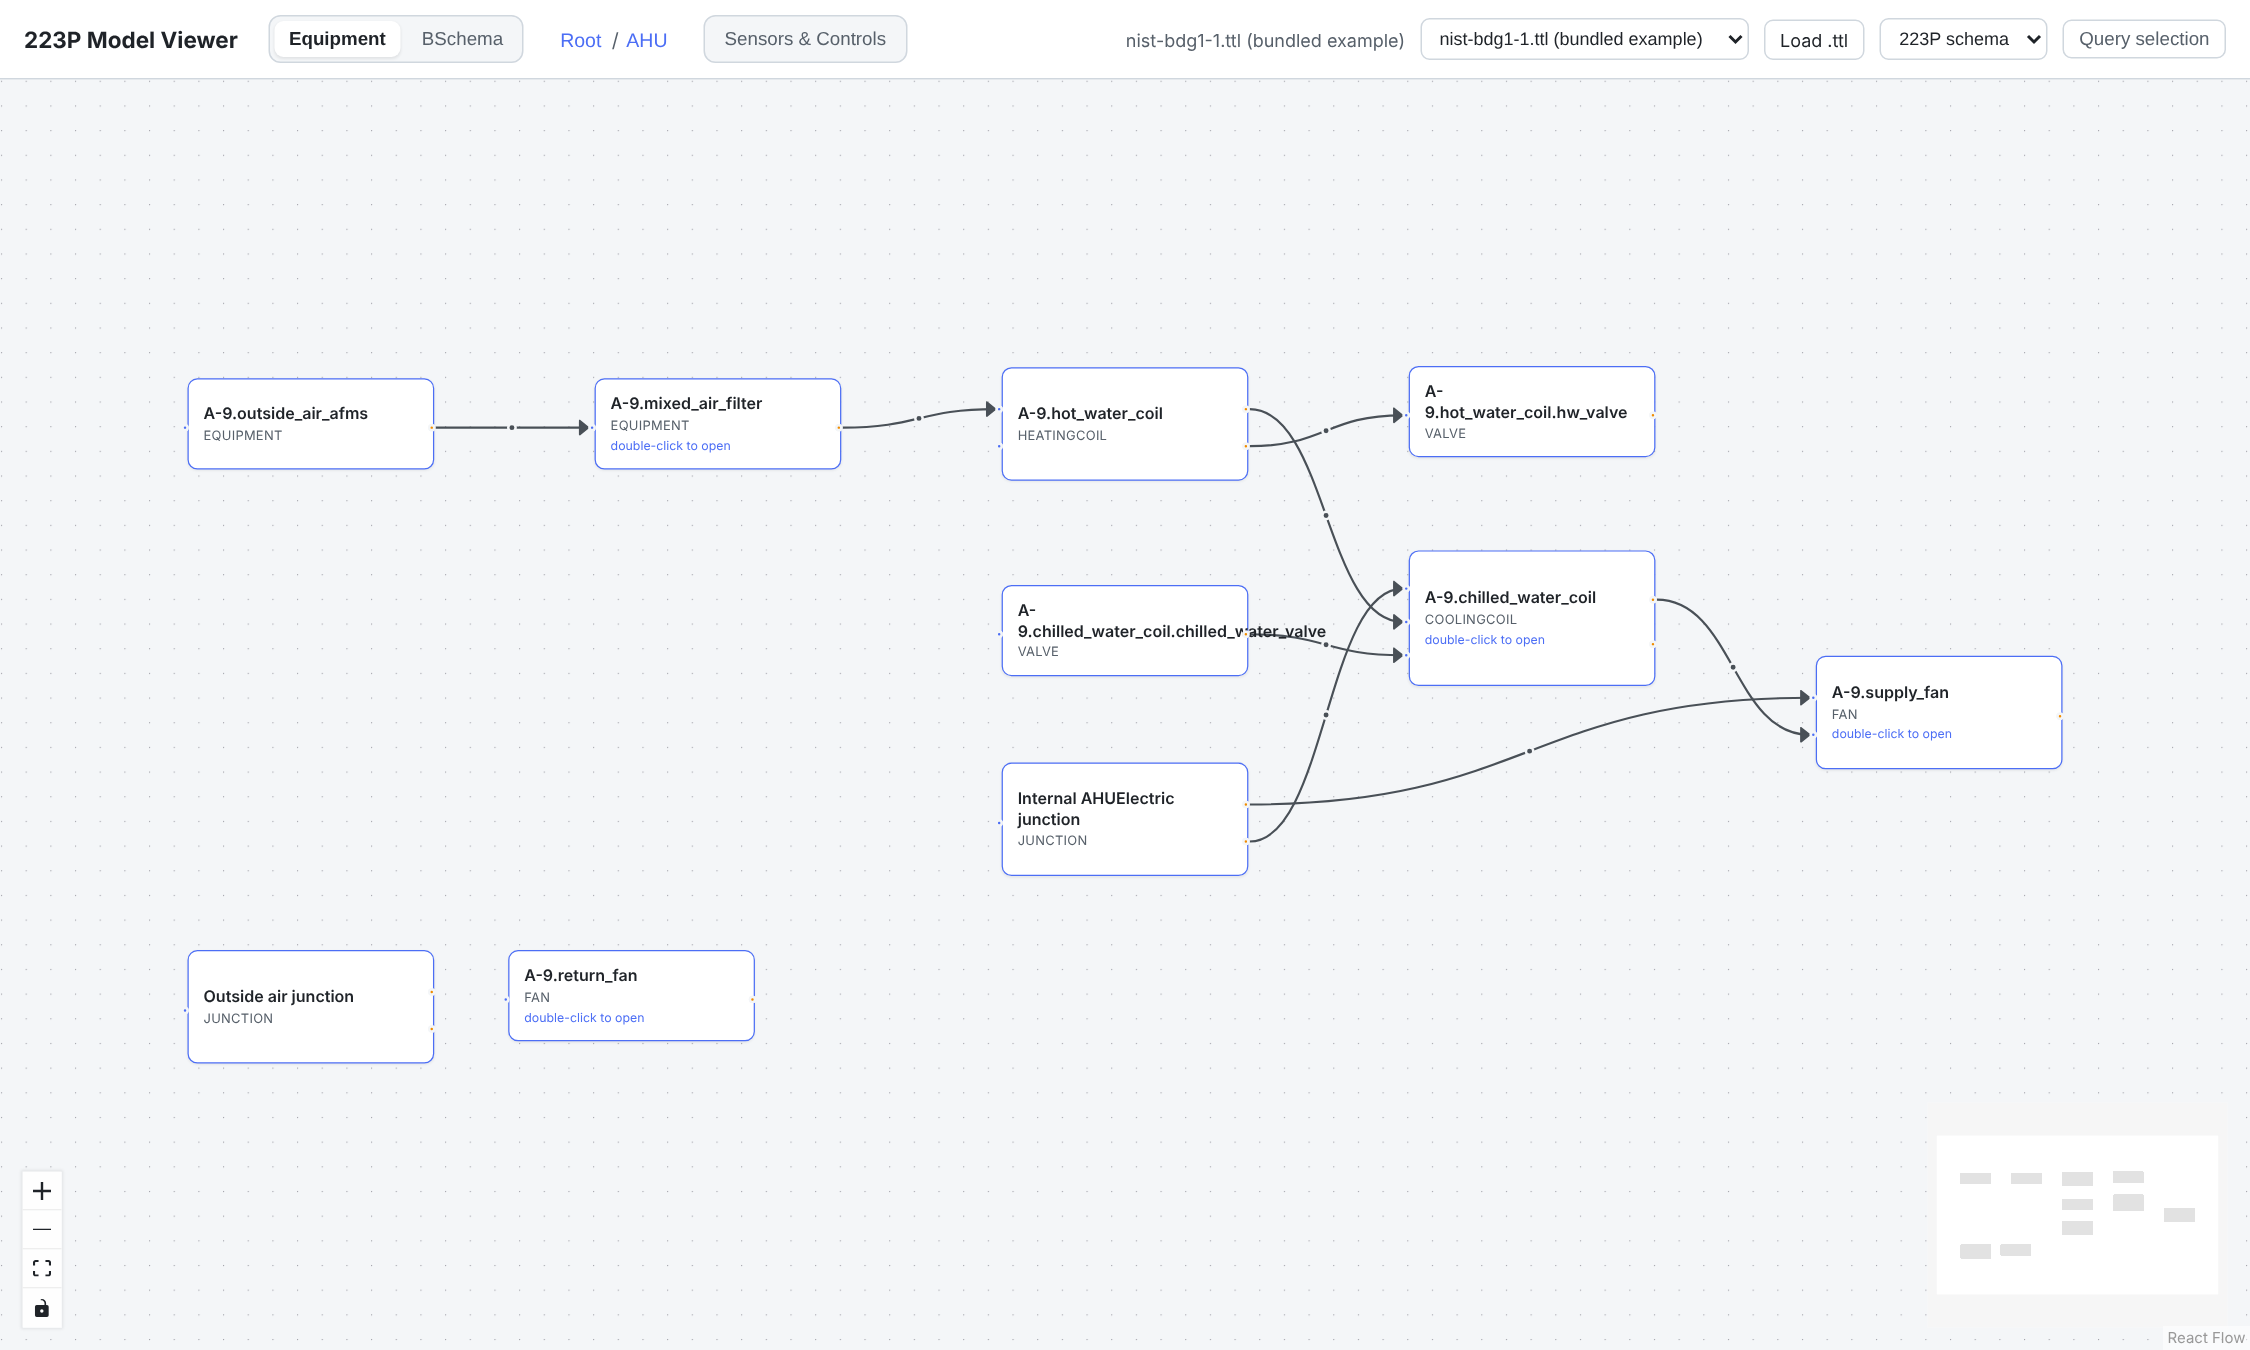
\includegraphics[width=0.49\textwidth]{../figures/fig-drill-ahu.png}
\caption{Left: root level of the NIST reference model (1{,}707 triples) as 25
boxes and 45 arrows; dashed arrows are rolled up (R5). Right: after
double-clicking the AHU, its internal components and their duct/pipe
connections; the breadcrumb reads \emph{Root / AHU}.}
\label{fig:root}\label{fig:drill}
\end{figure*}

Real data under-specifies containment, especially for instrumentation. A sensor
that \pred{observes} a property owned by a VAV box but is never
\pred{contains}'d anywhere would otherwise become a stray root. We therefore add a
\emph{functional parent} fallback, used only for nodes with no structural parent:
first the owner of a property the node observes, actuates, inputs, or outputs
(resolving through a connection point if the property is owned by one), then an
observation/physical location or actuated equipment, then the equipment that
\pred{executes} a function. Exactly one parent is chosen, preserving the tree.
In the reference model, 20 of the 70 tree edges come from this fallback.

\subsection{R5: Roll edges up to the nearest visible ancestor}
Most real 223P connections cross container boundaries: a luminaire's circuit runs
to a breaker in a different panel; a VAV's hot-water inlet runs to a boiler
outside every space. A strict ``draw an edge only if both endpoints are visible''
rule makes most of a building look disconnected. Instead, each connection
endpoint is walked up the containment tree to the nearest ancestor visible at the
current level. Edges that land on their true connection points are drawn solid
and port-to-port; edges with at least one projected endpoint are drawn dashed and
attached to the box rather than a port, and parallel projected edges between the
same visible pair are merged into one arrow labelled ``$n$ connections''. At the
reference model's root, 19 of 45 arrows are rolled up; at the real building's
root, 68 of 320 are rolled up and 31 are merges. This is the main mechanism by
which the viewer avoids \emph{silently} dropping information while still showing
one level at a time.

\subsection{R6: Logical groups are annotations, not containers}
\pred{System} (\pred{hasMember}) and \pred{Zone} (\pred{hasDomainSpace}) are
arbitrary groupings that can cross physical boundaries. They are never drawn as
boxes; each member's tooltip lists ``member of \emph{System}''. This is the
outcome of four design iterations, discussed in \cref{sec:systems}.

\subsection{R7: Hide instrumentation and scaffolding by default}
In the plain equipment view, nodes with core instrumentation relations (sensors,
actuators, functions, controllers) are not drawn, and any edges are routed around
them; uncontained instrumentation never becomes a root. The file's
\pred{owl:Ontology} declaration, untyped blank nodes, and external references are
likewise excluded. Instrumentation is not lost; it is the content of an overlay
(\cref{sec:overlay}).

% ---------------------------------------------------------------------------
\section{Progressive Disclosure}
\label{sec:disclosure}

Reduction decides what the default view is; disclosure decides how the user gets
to everything else without the default view paying for it.

\subsection{Sensors \& Controls overlay}
\label{sec:overlay}
An early version had a separate, flat ``points'' canvas. It answered ``what
sensors exist'' but not ``where are they'', so it was merged into the equipment
view as a toggle that \emph{overlays} the containment hierarchy
(\cref{fig:overlay}). With the toggle on:

\begin{itemize}[leftmargin=*,itemsep=1pt]
  \item Sensors, actuators, functions, and controllers appear as boxes with a
  color-coded border and a kind badge.
  \item Each property a point observes, actuates, inputs, or outputs appears as a
  rounded \emph{pill} (deduplicated, so two points sharing a property share a
  pill), wired point$\to$pill and pill$\to$owning box, with owner edges rolled up
  as in R5. Location, executor, and actuated-equipment links draw straight to the
  target box.
  \item Boxes with neither properties nor instrumentation of their own are
  \emph{muted}---shrunk and greyed---so the eye goes to what carries data while
  the structural context remains.
  \item Points are pulled in by \emph{attachment}, not only by tree position: a
  point anywhere in the model is included if it is a child here, if one of its
  location/executor links resolves to something visible here, or (in a single
  bounded second pass, not a fixed-point closure) if it targets a property that
  already has a pill. This recovers functions whose input/output properties have
  no declared owner, a common pattern in real data.
  \item Three sub-toggles gate the volume: \emph{Sensors \& Actuators} (on by
  default), \emph{Functions} (off by default, since real models can declare many),
  and \emph{All Properties} (off by default; surfaces every property owned by a
  visible box, even uninstrumented ones).
  \item Properties owned by a \pred{Connection} itself (e.g.\ a mixed-air duct
  temperature) cannot attach to either endpoint. With \emph{All Properties} on,
  the arrow is split by a small junction dot and the pill wires to the junction---
  the closest node-link analogue of ``an edge pointing at an edge''.
  \item Links that cannot be drawn because their target is the container one is
  currently inside are listed in the point's tooltip instead of being dropped.
\end{itemize}

\begin{figure}[t]
\centering
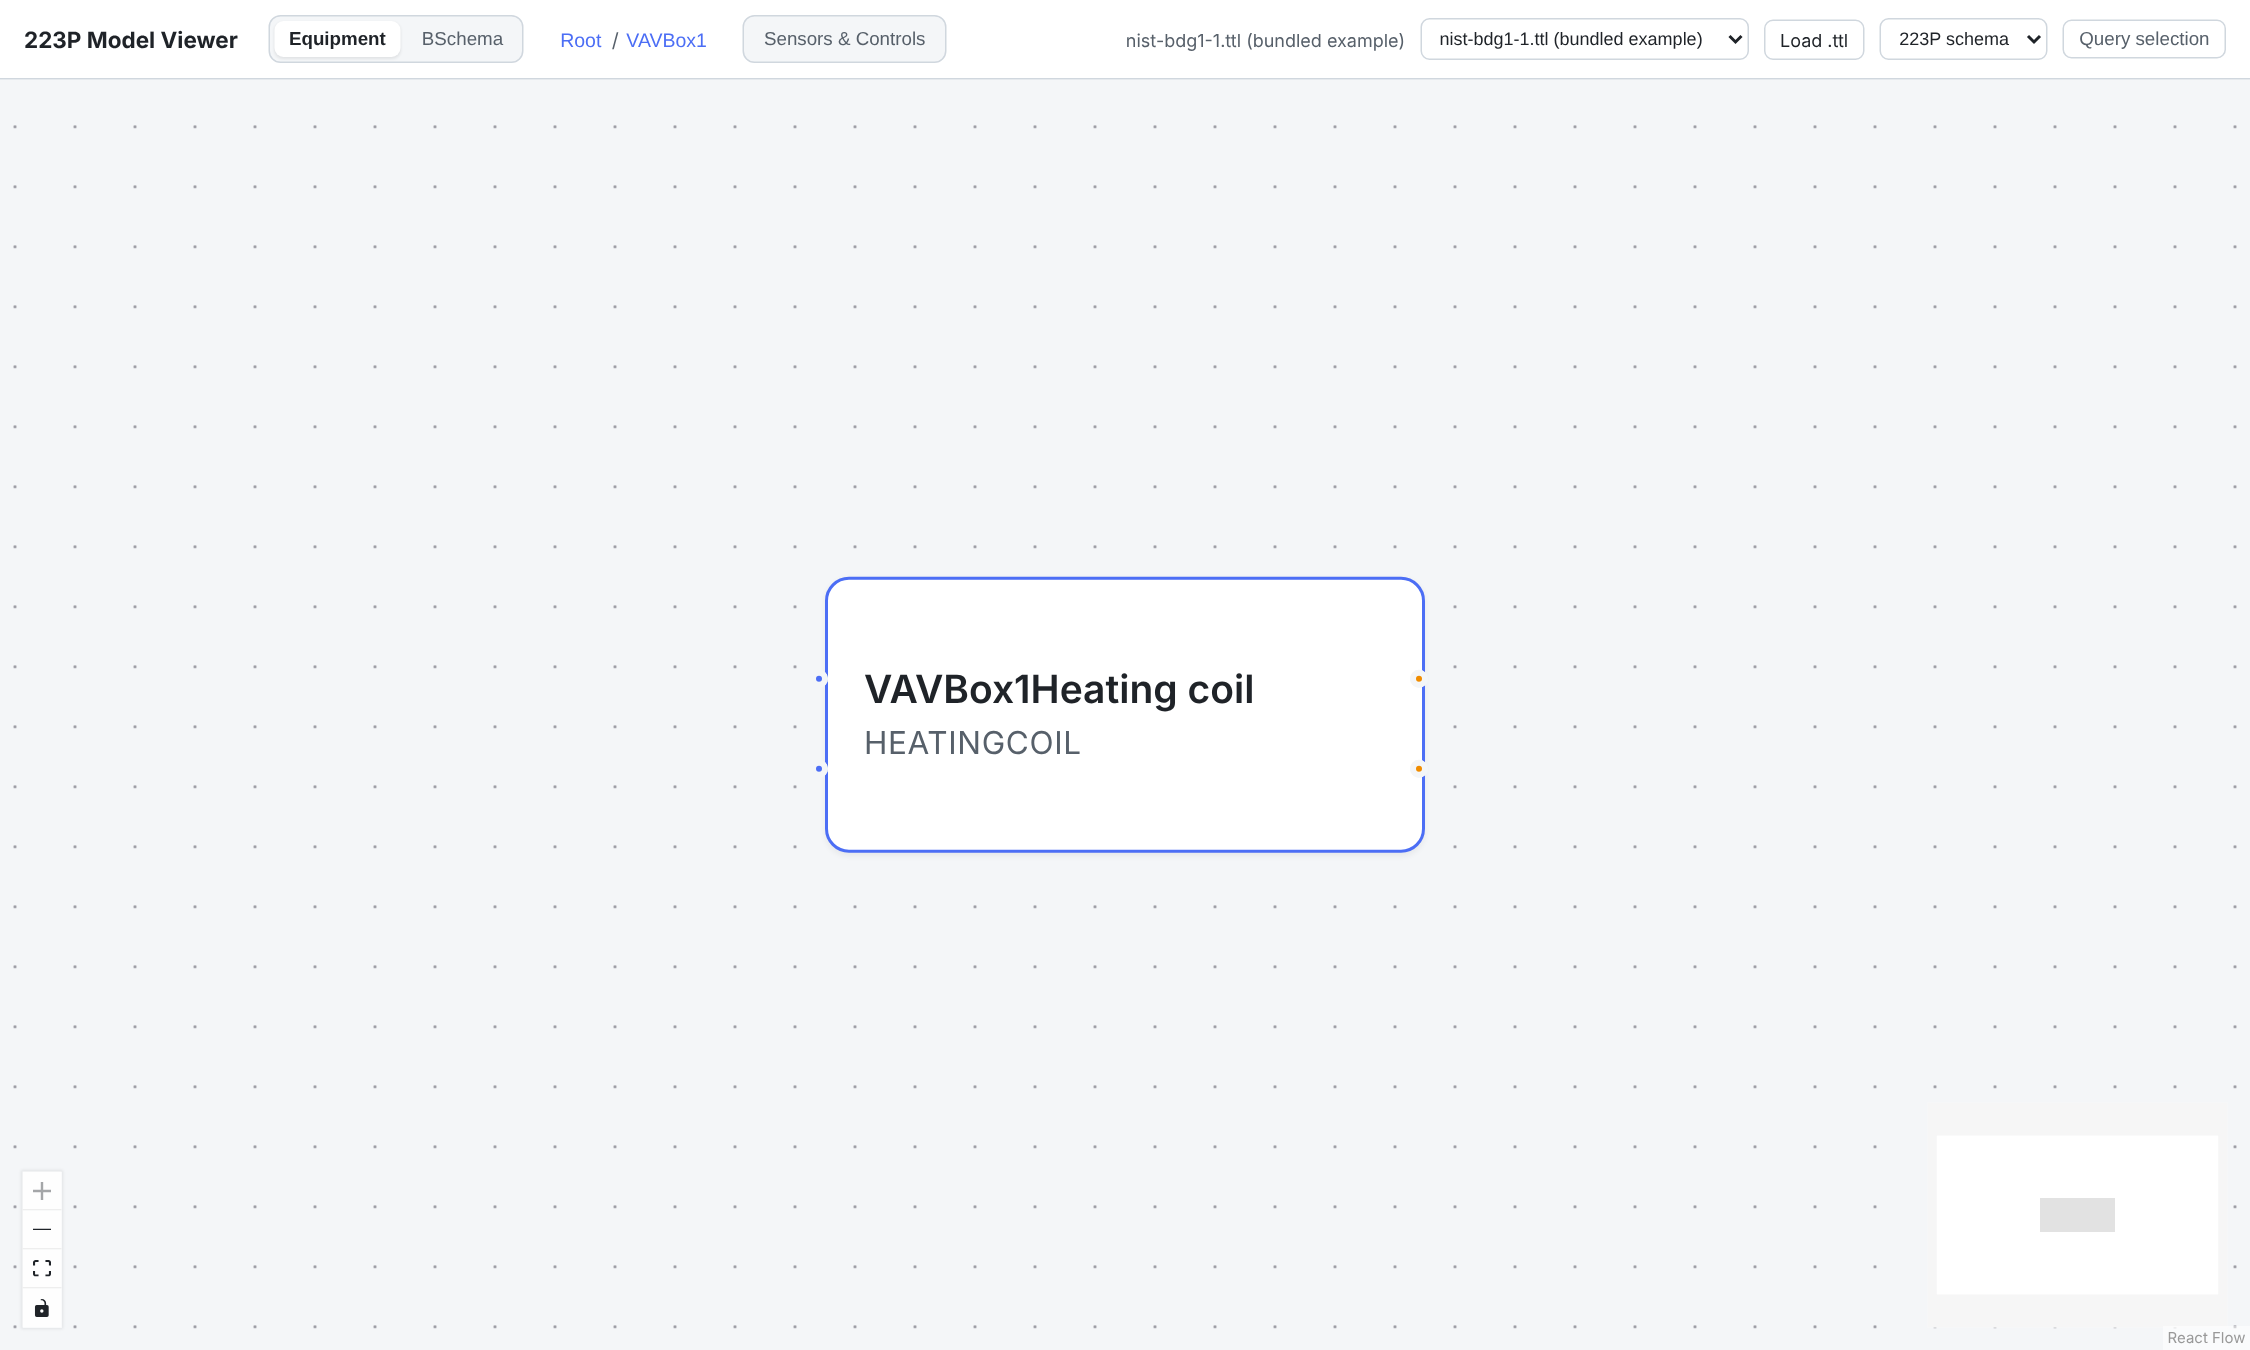
\includegraphics[width=\linewidth]{../figures/fig-vav-plain.png}\\[2pt]
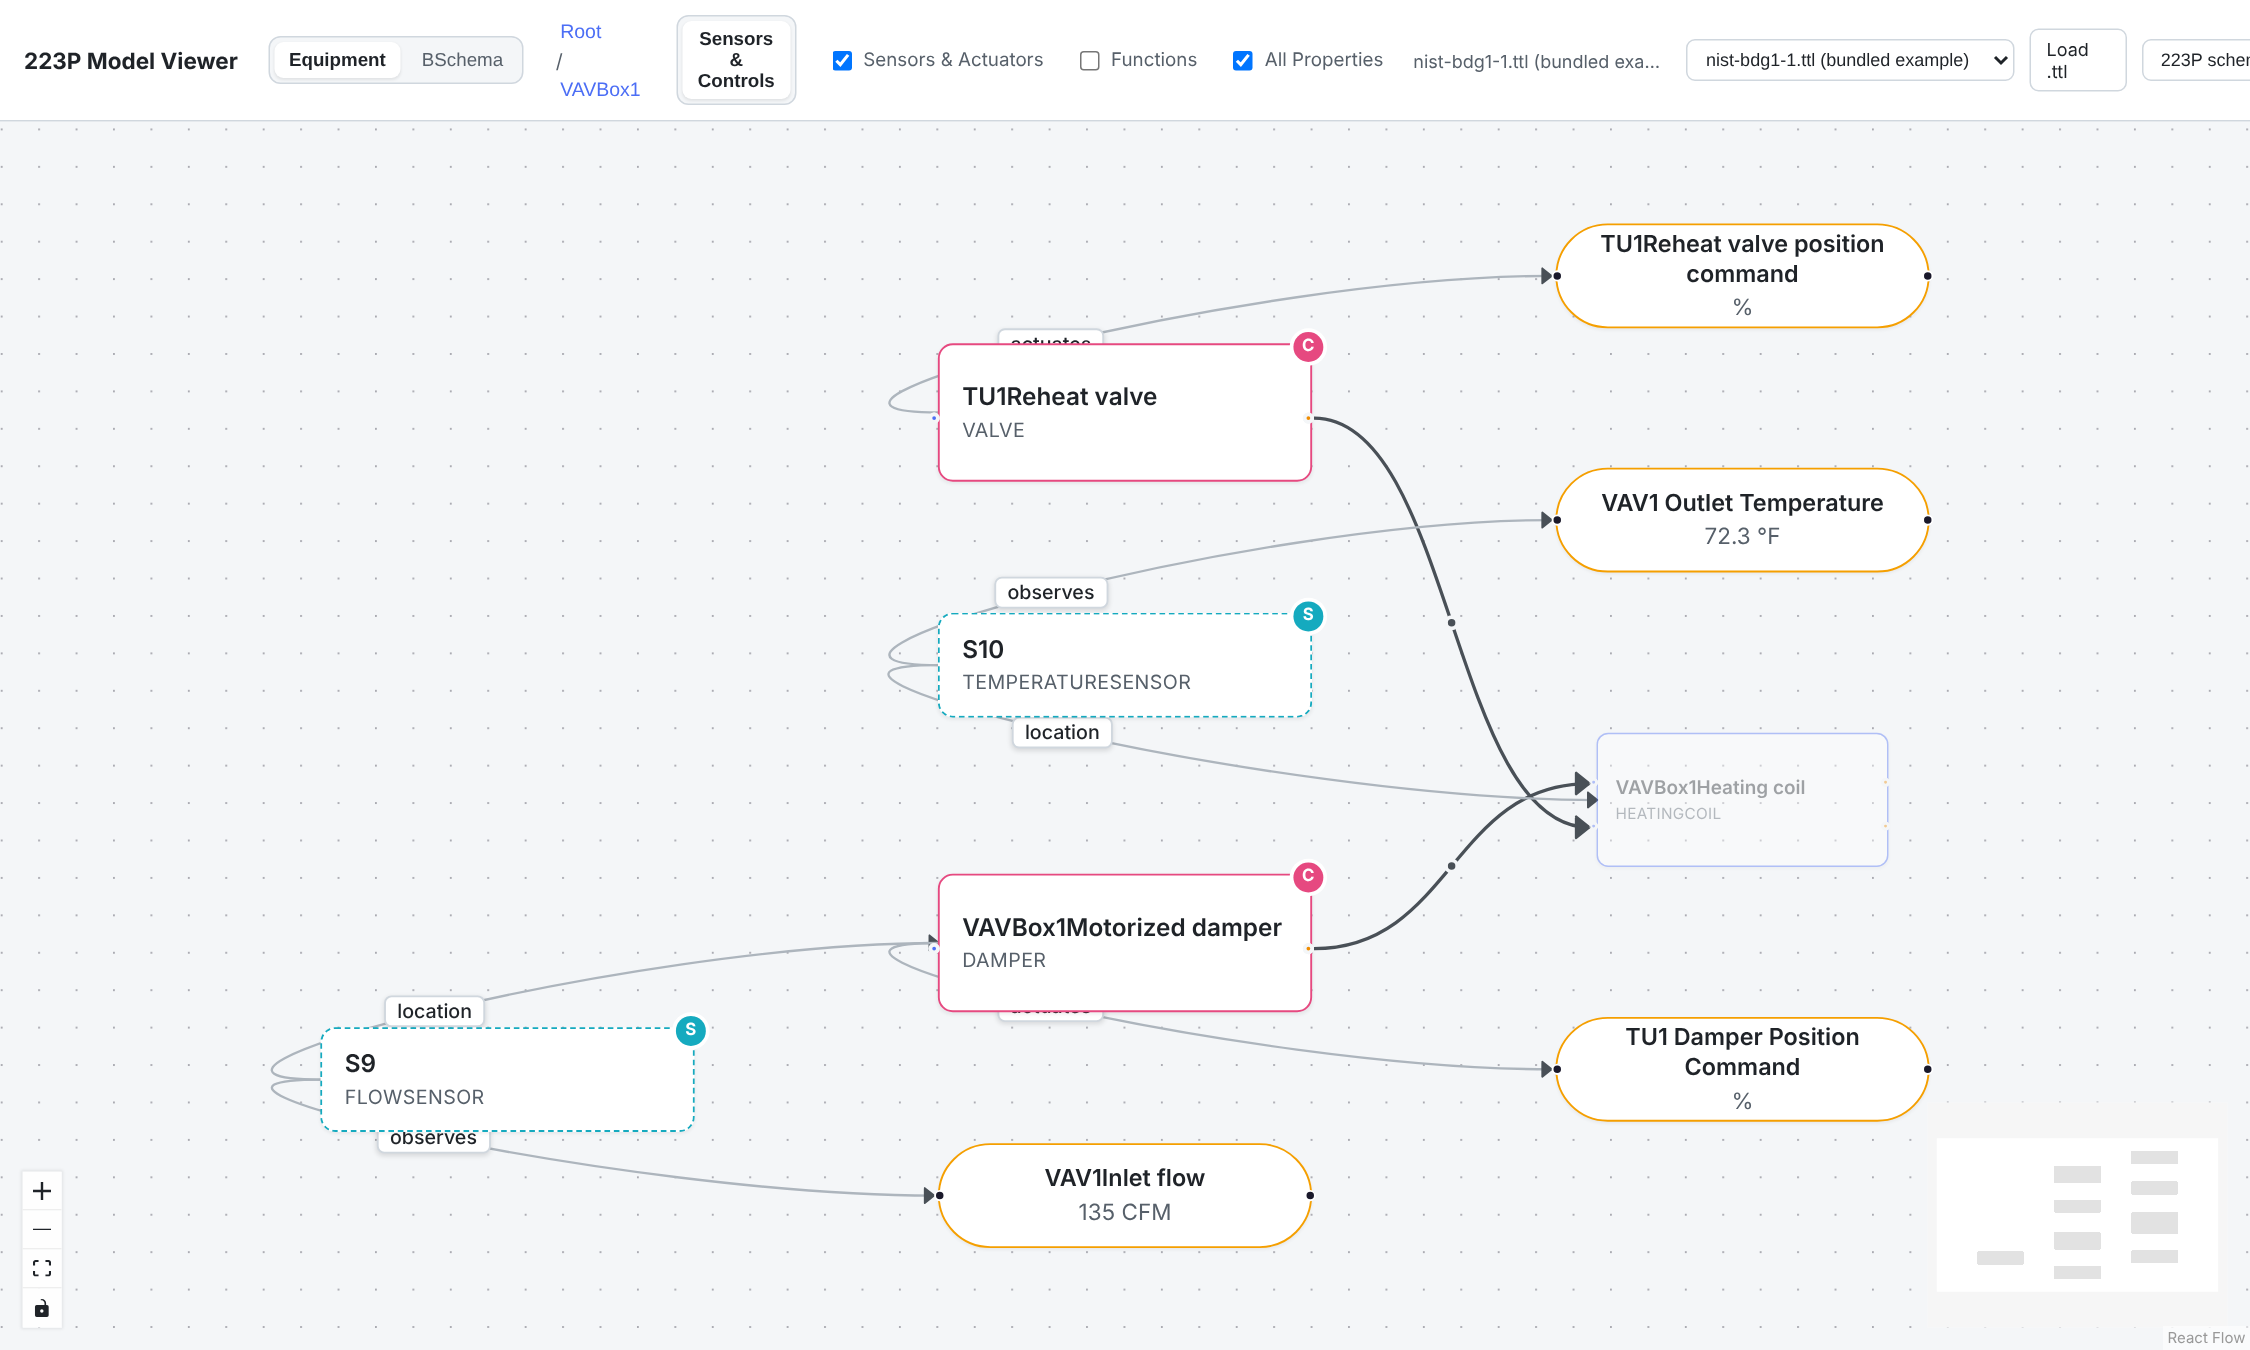
\includegraphics[width=\linewidth]{../figures/fig-vav-overlay.png}
\caption{Inside VAVBox1. Top: plain equipment view, showing only the heating coil.
Bottom: Sensors \& Controls with All Properties---sensors (S) and actuated
equipment (C) as bordered boxes, property pills with values and units, labelled
instrumentation edges, and the property-less heating coil muted. The reheat valve
and damper are hidden in the top view because they carry actuation relations
(\cref{sec:limits}).}
\label{fig:overlay}
\end{figure}

\subsection{Schema summary as an entry point}
For large buildings even the root level is dense (\cref{sec:limits}). We
therefore support starting from a \emph{schema summary}: a class graph produced by
an external summarization tool that buckets structurally similar instances of a
building into versioned classes (e.g.\ \texttt{AirHandlingUnit\_version\_1},
\texttt{FanPoweredTerminal\_version\_1}). Because that summary is itself
expressed in 223P, it renders through the same pipeline with no special code
(\cref{fig:bschema}). For the real building, 30 summary nodes (8 at the root)
stand in for 66 member lists covering 4{,}604 instance links. Hovering a class
lists its real members; clicking one switches to the instance view, loads the
building, drills to the member's parent, turns on the overlay, and highlights and
focuses the target box. The summary thus functions as an overview from which
the user drills into detail, rather than as a separate tool.

\begin{figure}[t]
\centering
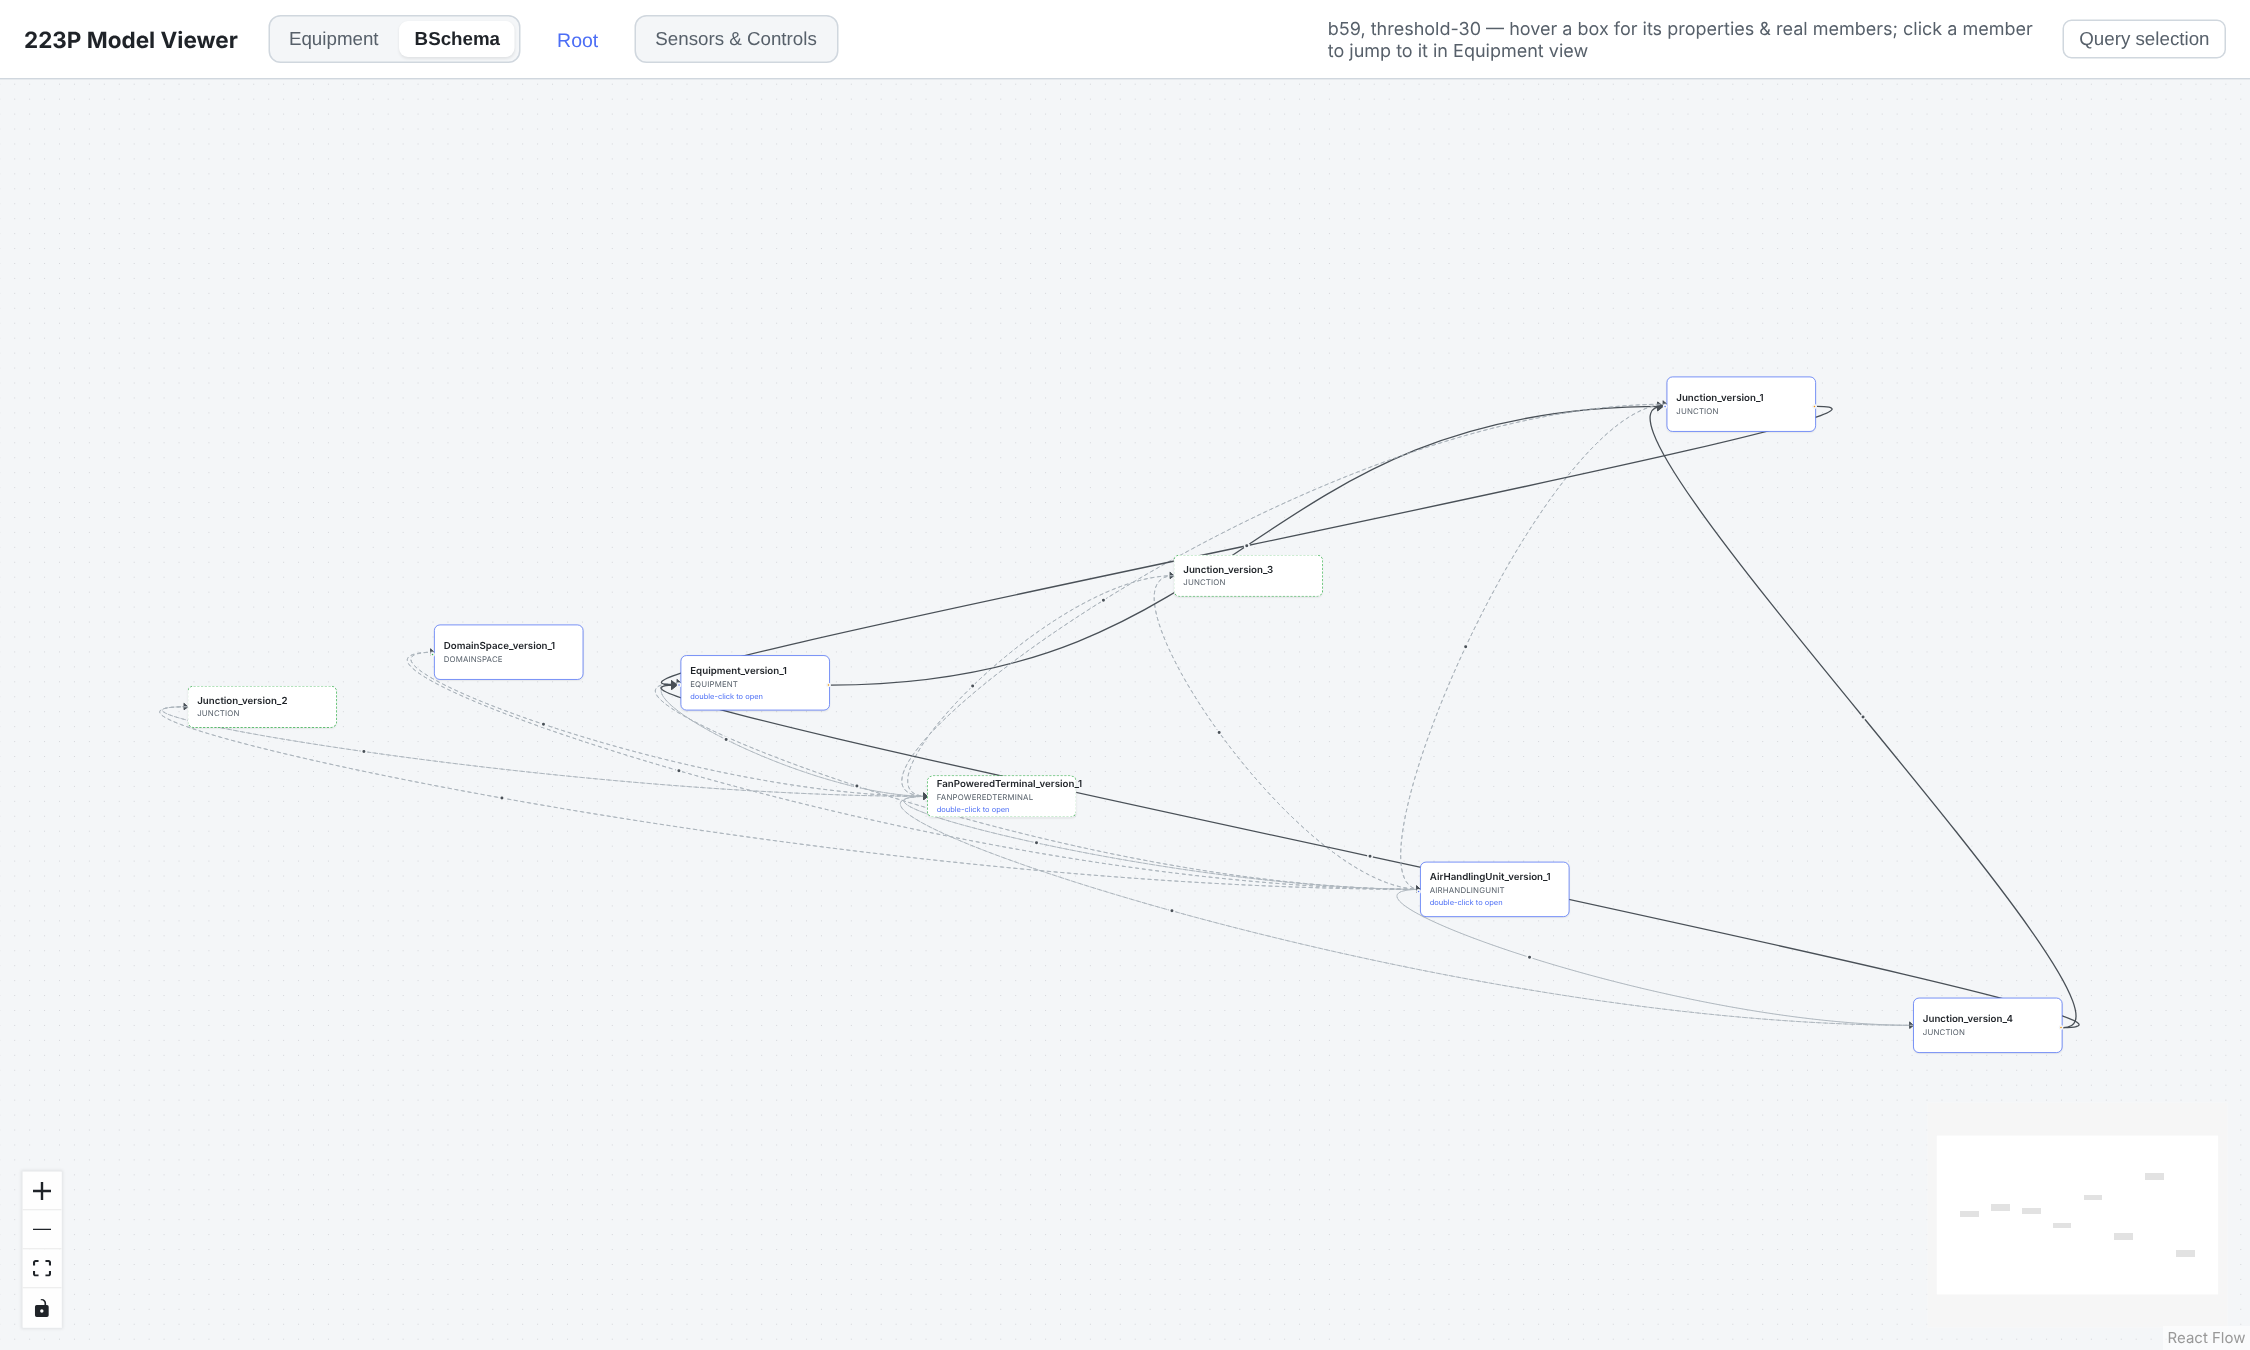
\includegraphics[width=\linewidth]{../figures/fig-bschema.png}
\caption{Schema-summary view of the real building: eight root classes instead of
143 root instances. Hovering a class lists its real members, each a link into
the instance view.}
\label{fig:bschema}
\end{figure}

\subsection{From looking to querying}
The viewer is also a query-construction aid. A \emph{query selection} sidebar
offers instances, classes, predicates, and literals drawn from what is in view---
the visible boxes plus everything their tooltips and arrows stand for, including
the real endpoints, ports, and hubs folded into a rolled-up arrow. Clicking
(shift-clicking for several) boxes narrows that scope to the selection. In the
notebook widget, a 223P-specific variant lets the user choose predicates to
traverse and then pick an instance, collecting every one-hop triple in which it
is subject or object on those predicates, queried against the full graph rather
than the visible subset. The resulting clipboard, a list of structured triples
with provenance, syncs back to Python, where it can seed a SPARQL query. The
reduced view thus also serves as an index into the full graph.

% ---------------------------------------------------------------------------
\section{Layout and Responsiveness}
\label{sec:layout}

\paragraph{Component-wise layout with shelf packing.}
Real building views are dominated by small disconnected clusters plus many
singletons. A single layered layout of the whole slice stacks the singletons into
an absurdly tall column. We lay out each connected component independently
(left-to-right dagre) and shelf-pack components into rows, tallest first.
Singletons skip dagre entirely, which alone made the real building's root
layout three to four times faster.

\paragraph{Crossing-minimization trials with a time budget.}
For components of eight or more nodes we increase spacing and run additional
dagre passes over randomly shuffled insertion orders, keeping the layout with the
fewest straight-line crossings between node centers. The unshuffled order is
always tried first so trials can only help, and a seeded PRNG keeps re-layouts
identical between renders. Because dagre's cost grows superlinearly (we measured
roughly 9\,ms at 10 nodes and 315\,ms at 143 nodes/320 edges), a 400\,ms
wall-clock budget caps the trials; the trial-count heuristic alone had permitted a
6-second stall on the real building.

\paragraph{Mark sizing.}
Box height grows with port count up to a cap, after which ports become denser
rather than boxes taller; junction dots are laid out at dot size so they do not
reserve an equipment-sized slot.

\paragraph{Interaction latency as clutter.}
A slow view is an overwhelming view. Selection and highlight originally sat in
the same memoized computation as layout, so every click re-ran layout; on the real
building with the overlay on (228 nodes), a shift-click blocked the main thread
for about 13.5\,s. Splitting layout (keyed only on graph shape) from a cheap
pass that stamps selection flags onto already-positioned nodes, and memoizing node
components, brought this to 150--200\,ms.

% ---------------------------------------------------------------------------
\section{Case Study: Where Do Systems Go?}
\label{sec:systems}

The hardest reduction decision was \pred{System}. It is tempting to draw a System
as a box containing its members---that is what ``system'' sounds like. But
\pred{hasMember} and \pred{contains} can independently claim the same node, and a
single-parent drill-down can honor only one. We went through four designs:

\begin{enumerate}[leftmargin=*,itemsep=1pt]
  \item \textbf{Every System is a box.} ``Return System'' (a return fan and an
  exhaust damper, both also \pred{contains}-children of the AHU) rendered as a
  disconnected box beside the AHU, its members' wiring hidden inside it.
  \item \textbf{Boundary-driven, then inferred.} A System became a box only if it
  declared \pred{hasBoundaryConnectionPoint}. We then added inference: if a strict
  majority of members already sat in one container, nest the System there as a
  logical group (``Supply System'' had 7 of 8 members inside the AHU; its one
  boundary port belonged to the eighth); otherwise, treat wiring that left the
  member set as an implied boundary. An \emph{Inferred/Literal} toggle switched
  between heuristics and pure RDF.
  \item \textbf{Display toggle.} \emph{Flat/Abstracted}: in Abstracted mode a
  majority-container System became a real drillable box inside that container,
  reparenting its members---the only place \pred{hasMember} overrode
  \pred{contains}. A softer alternative, dashed ``cluster frames'' drawn around
  members in the flat layout, was tried and rejected: in use we preferred something
  they could open, and because the layout knows nothing of membership, frames
  could overlap one another and enclose non-members.
  \item \textbf{Always logical (current).} Systems and Zones are never boxes,
  even with real boundary ports (a breaker panel with six). Membership is
  hover text on each member; members appear wherever physical containment puts
  them.
\end{enumerate}

The final step was not a bug fix but a deliberate simplification: one fewer
decision surfaced to the user, one axis of behavior removed from the code, and
no heuristics whose thresholds would need tuning per building. The richer
implementations are preserved under a version-control tag rather than kept
behind a toggle. We regard this as the central lesson of the project: when two
relations both claim to be the hierarchy, \emph{pick one and annotate with the
other}.

% ---------------------------------------------------------------------------
\section{Design Principles}
\label{sec:principles}

\begin{enumerate}[label=\textbf{P\arabic*},leftmargin=*,itemsep=2pt]
  \item \textbf{Draw the domain's things, not the triples.} Map ontology patterns
  to the marks an engineer would draw: boxes, ports, arrows, and lists. Do this in
  a shared domain model, before layout (R1--R3).
  \item \textbf{One tree, one relation.} Let exactly one family of relations
  (physical containment) define position. Other groupings become annotations
  (R4, R6, \cref{sec:systems}).
  \item \textbf{Nothing vanishes silently.} When something cannot be shown at
  this level, show it in summarized form: a dashed rolled-up arrow, a merged
  ``$n$ connections'' label, a tooltip line (R5, \cref{sec:overlay}).
  \item \textbf{Be faithful, not clever.} Infer only from relations the standard
  defines. We twice reverted heuristics that guessed structure from names or
  incidental properties (e.g.\ treating anything named \texttt{*Sensor} or
  carrying a unit as a Brick Point). A faithful view makes data gaps visible
  instead of papering over them (\cref{sec:findings}).
  \item \textbf{Conservative defaults, opt-in detail.} Instrumentation, functions,
  and uninstrumented properties are off by default and one click away.
  \item \textbf{Removing options is a feature.} Each toggle is a decision pushed
  onto the user and a code path to maintain. Prefer one good default
  (\cref{sec:systems}).
  \item \textbf{One pipeline, many inputs and hosts.} Brick models, schema
  summaries, and notebook embedding all reuse the same model and renderer, so
  reduction behavior stays consistent across them.
  \item \textbf{Latency is part of clutter.} Keep layout off the interaction path.
  \item \textbf{Serve many mental models from one model, and keep the bridges.}
  Give each kind of user a lens that matches how they think, over a shared model
  so that the same entity can be followed from one lens to another
  (\cref{sec:lenses}).
\end{enumerate}

P4 has one acknowledged tension: presentation-level choices (color-coding a node
as a sensor, and excluding uncontained instrumentation from the root) use type-name
suffixes. These affect styling and default visibility, never structure or
ownership.

% ---------------------------------------------------------------------------
\section{Descriptive Evaluation}
\label{sec:eval}

We have not yet run a user study (\cref{sec:limits}). Here we report how much the
reduction shrinks four bundled models, and what using the viewer revealed about
the models themselves.

\begin{table*}[t]
\centering
\small
\caption{Reduction on the bundled models. ``RDF nodes'' are distinct subjects and
objects. Root boxes and arrows are the default (overlay off) root view; rolled-up
arrows are those with at least one endpoint projected to a visible ancestor
(R5). The overlay column is the root view with every overlay toggle on (boxes /
added pills and junctions).}
\label{tab:stats}
\begin{tabular}{lrrrrrrrrr}
\toprule
Model & Triples & RDF nodes & Equip./space & Hubs & CPs & Props/points & Conn.\ arrows & Root boxes / arrows (rolled) & Overlay \\
\midrule
NIST reference (223P) & 1{,}707 & 432 & 111 & 50 & 146 & 65 & 88 & 25 / 45 (19) & 28 / 15 \\
Real building B59 (223P) & 38{,}982 & 4{,}646 & 620 & 518 & 1{,}612 & 1{,}803 & 542 & 143 / 320 (68) & 196 / 754 \\
BOPTEST-derived (Brick) & 985 & 181 & 13 & -- & 24$^\dagger$ & 72 & 12 & 13 / 12 (0) & -- \\
B59 schema summary & 848 & -- & 30 & -- & 17 & -- & 338 & 8 / 96 & -- \\
\bottomrule
\end{tabular}

\smallskip
{\footnotesize $^\dagger$Synthetic ports created for \pred{feeds} edges. Equip./space
excludes hubs and logical groups (12 in NIST, 51 in B59). Parse + model build:
44\,ms (NIST) and 364\,ms (B59) in Node.js.}
\end{table*}

\paragraph{Reduction.}
For the NIST reference model, a view of 25 boxes and 45 arrows stands in for
432 RDF nodes and 1{,}707 triples at the root, with maximum containment depth 3
(\cref{tab:stats}). Brick reduces to 13 boxes and 12 arrows with all 72 points in
tooltips. For the real building, the reduction is larger in absolute terms
(38{,}982 triples to 143 boxes) but the result is still too dense to read
(\cref{fig:b59}), because the export leaves most equipment uncontained (maximum
depth 2). Turning every overlay toggle on at that root adds 754 pills and
junctions---exactly the case the conservative defaults (P5) are meant to avoid.

\begin{figure}[t]
\centering
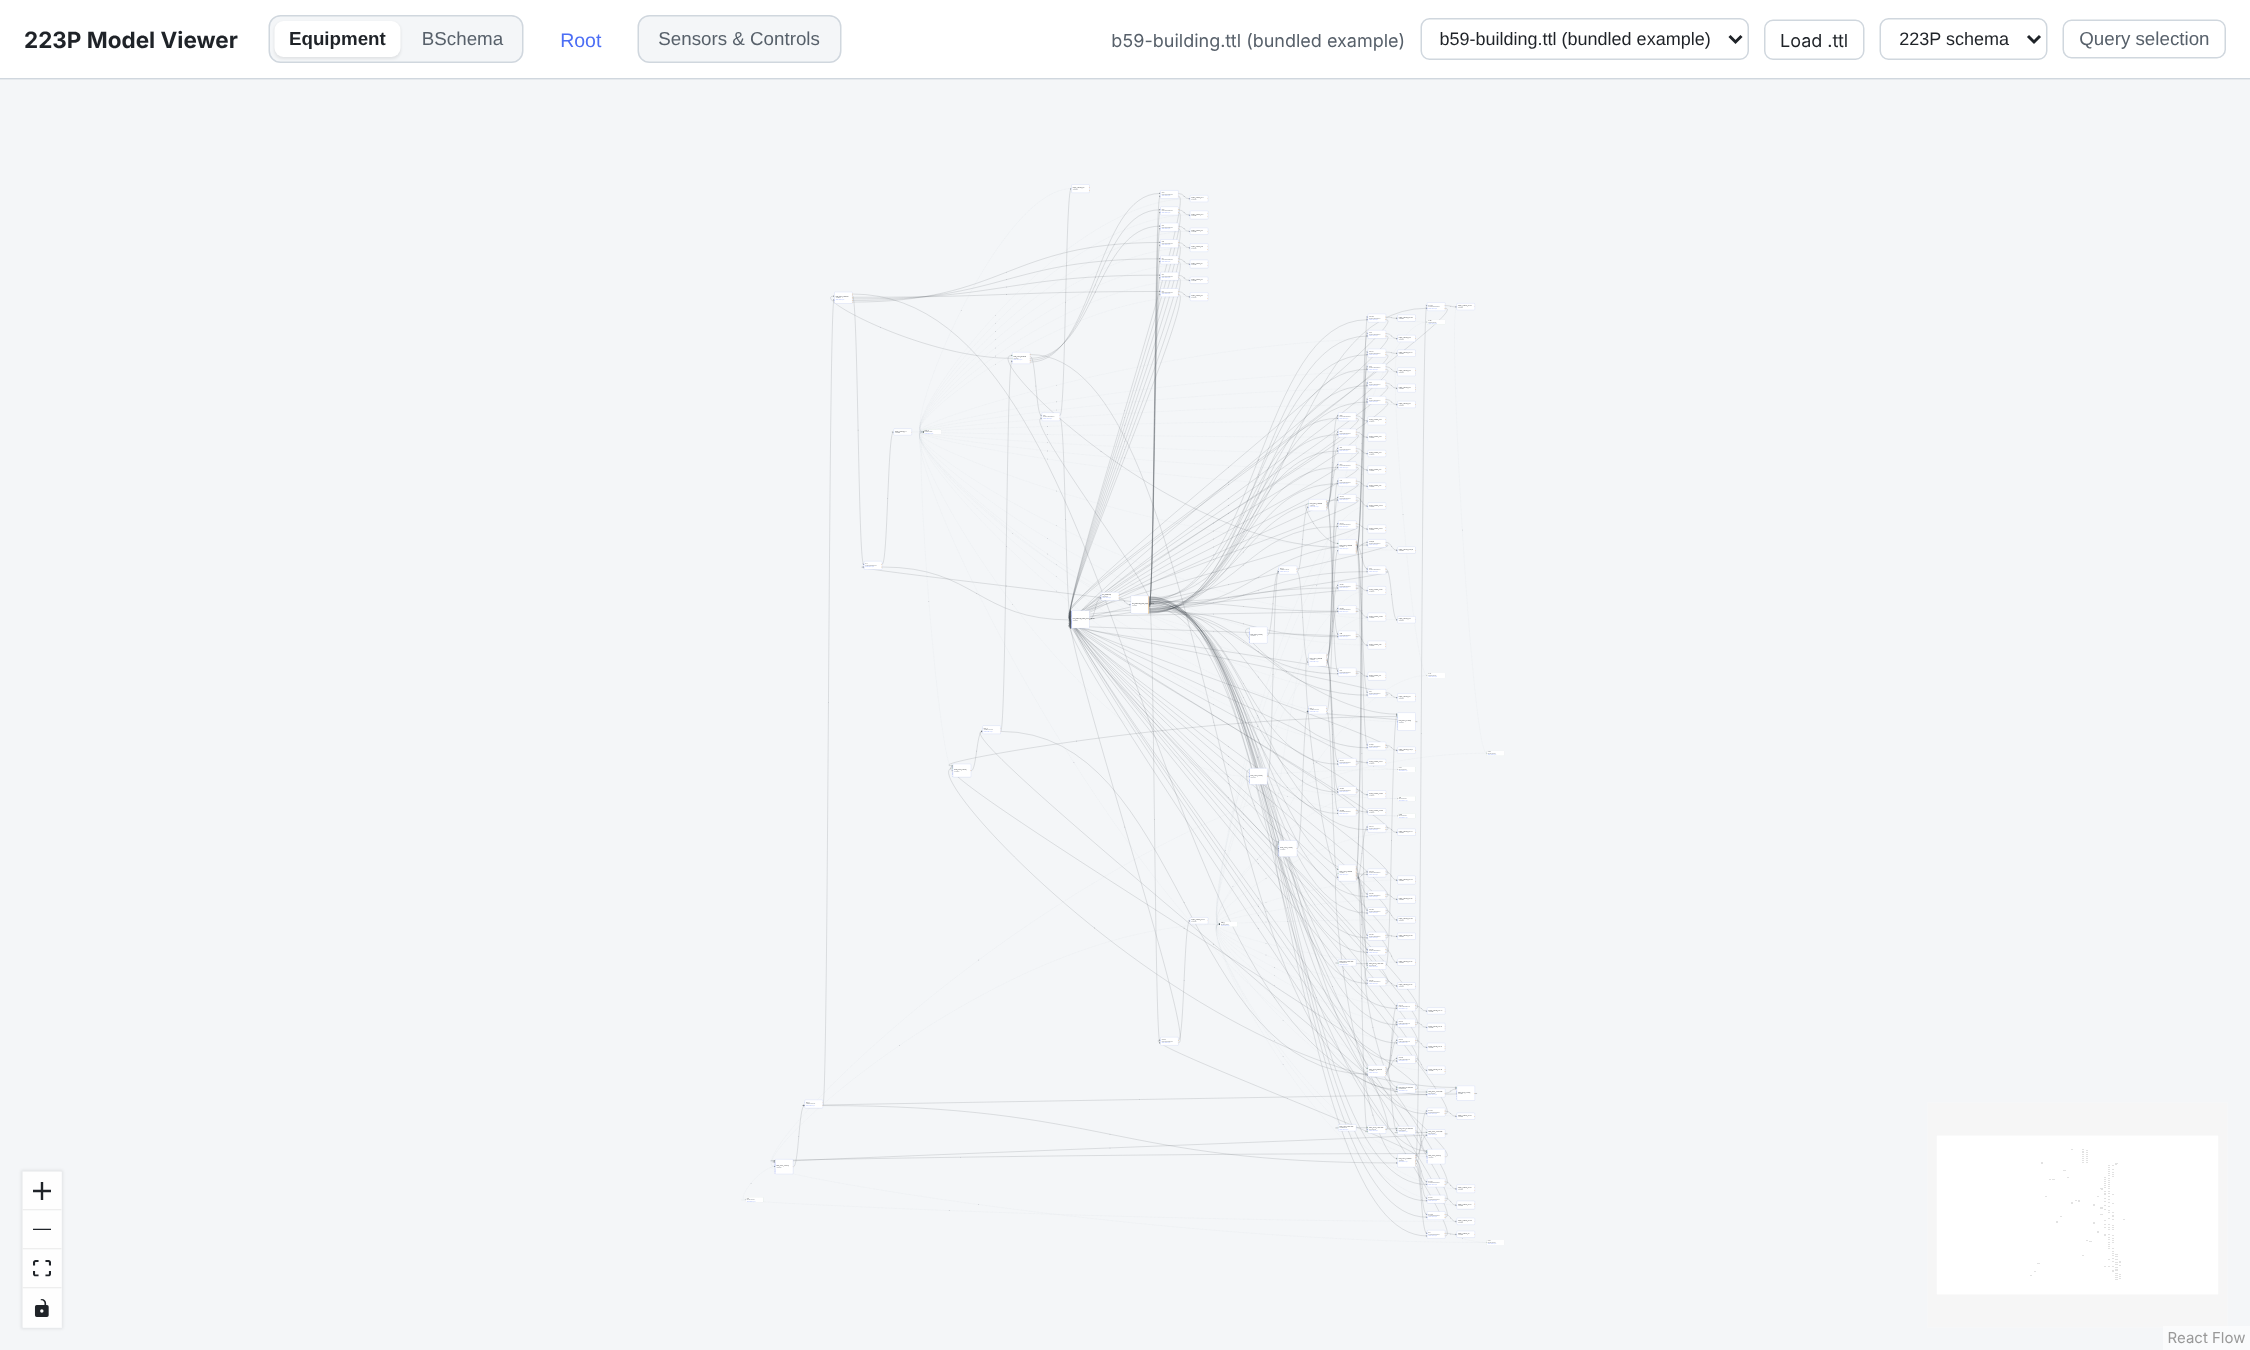
\includegraphics[width=\linewidth]{../figures/fig-b59-root.png}
\caption{The real building's root view: 143 boxes and 320 arrows. Semantic
reduction alone is not enough when the source model declares little
containment; the schema-summary view (\cref{fig:bschema}) is the better entry
point here.}
\label{fig:b59}
\end{figure}

\paragraph{The viewer as a model checker.}
\label{sec:findings}
Because the viewer refuses to guess (P4), modeling errors show up as visual
anomalies. Examples from development:
(i) a flow sensor in VAV box 1 whose observation location pointed at VAV box 2's
damper inlet---a copy-paste error that appeared as a property pill floating
disconnected inside VAV box 1;
(ii) a Brick model whose heat pump, chiller, and five zone CO$_2$ sensors lacked
\pred{feeds}/\pred{hasPoint} links and so appeared as disconnected boxes instead
of folding into their equipment;
(iii) summary-graph connection points claimed by many owners, which exposed a
viewer bug (keeping only the first owner) that had also silently dropped two
breaker-to-luminaire circuits in the reference model.
Cases (i) and (ii) were fixed in the source data rather than worked around in
the viewer.

% ---------------------------------------------------------------------------
\section{Limitations and Future Work}
\label{sec:limits}

\begin{itemize}[leftmargin=*,itemsep=1pt]
  \item \textbf{No user study.} Our claims about comprehension are design
  rationale and practitioner feedback, not measured outcomes. A task-based
  study (e.g.\ ``which sensors affect VAV-3's discharge temperature?'') against a
  generic RDF browser and a tabular baseline is the natural next step.
  \item \textbf{Few models.} Four bundled models, one of each kind. Systems
  behavior in particular has been exercised on one model with four Systems.
  \item \textbf{Flat exports stay dense.} When containment is sparse, R4 has
  little to work with (\cref{fig:b59}). Candidate remedies are automatic entry
  through the schema summary, degree-of-interest filtering~\cite{vanham2009search},
  or a containment-inference step clearly marked as inferred.
  \item \textbf{Hard-coded semantics, two ontologies.} Mappings are written for
  223P and Brick; \cref{tab:ontologies} is analysis, not implementation. Expressing
  the mappings declaratively (e.g.\ as SHACL-annotated view rules) would make them
  inspectable and portable to Haystack, RealEstateCore, or BOT-based models, and
  would let a model combining several ontologies feed every lens at once.
  \item \textbf{Missing lenses.} There is no dedicated spatial lens (``what serves
  this room?''); spaces appear only as containers in the topology lens. Nor have we
  tested which lens each user group actually reaches for first; the personas in
  \cref{tab:lenses} are hypotheses to be checked in a study.
  \item \textbf{Actuated equipment counts as instrumentation.} R7 hides any node
  with a core instrumentation relation. Valves and dampers that declare
  \pred{actuatedByProperty} therefore vanish from the plain equipment view
  (\cref{fig:overlay}, top) even though they are physical equipment with ports.
  Restricting R7 to nodes without connection points would fix this.
  \item \textbf{Systems remain text.} Always-logical Systems are simple and
  honest, but a user asking ``show me the supply system'' still has no direct
  view. A membership-aware highlight (rather than a box) is a candidate that
  would keep P2 intact.
\end{itemize}

% ---------------------------------------------------------------------------
\section{Conclusion}

Semantic building models are now detailed enough to be hard to look at, and part
of the reason is that they describe the building for several kinds of user at
once. Our experience building 223p-viewer suggests treating that as a strength:
serve each mental model as its own lens over one shared model, connect the lenses
so a user can cross between them, and let the ontology decide what each lens
draws---which nodes are things and which are scaffolding, which relation is the
hierarchy, and which relations are annotations. Using that knowledge before layout,
revealing the rest on demand, and resisting heuristics that guess beyond the data
together produced views that engineers can read and that also expose errors in the
models they depict.

\paragraph{Availability.}
Source code, bundled models, and the notebook widget:
\url{https://github.com/lazlop/223p-viewer}.

\bibliographystyle{plain}
\bibliography{refs}

\end{document}
